\documentclass[../main.tex]{subfiles}
\begin{document}

\section{Discussion}
\subsection{Gene Organization}

Variation in gene arrangement is not uncommon in demonsponges. Previous research from this lab showed that G0 and G1 orders were highly variable, but that G3 and G4 orders, of which Clade B is a part of G3, were much more conserved. In G3, protein-coding gene order is maintained with little deviation, and what variation that does exist can be contributed to the movement or loss of mitochondrial tRNA genes. However, the results of this study showed a unique gene arrangement in \emph{Niphates digitalis} and \emph{Niphates erecta} not in other demosponges.

At some point since the split of \emph{N. digitalis} and \emph{N. erecta} from \emph{A. queenslandica}, the \emph{Niphates} species underwent extensive genomic rearrangement, with clusters being flipped, relocated, or inserted into other clusters. As none of these rearrangements are seen in other demosponges and especially not in Clade B, it is mostly the result of a recent upset in this branch of the Clade B phylogeny. As this upset is not reflected in the mt-genomes of the other species with missing genes and the inverted repeats, the rearrangement most likely did not lead to the relocation of \emph{atp9} to the nuclear genome or cause the inverted repeats and insertions. It could have contributed to the multiple mt-tRNA gene losses seen in \emph{Niphates} and the relocation of \emph{atp8}, but as not every species that is missing mt-tRNAs has a novel genome arrangement, genome rearrangement events do not explain the loss of mitochondrial tRNA genes. Sequencing of additional species in Clade B would allow for a better understanding of \emph{Niphates} genome rearrangement event and could possibly elucidate the order in which the changes took place.

\subsection{Gene Content}
\subsubsection{Movement of \emph{atp9} and to the nuclear genome}
Gene loss is not uncommon in the history of mitochondrial genomes, and this is reflected in non-uniform gene content in mt-genomes across all branches of life. However, amongst demosponges, mitochondrial genomes display similar gene content. This is particularly true within the G3 and G4 orders of demosponges, which have an accepted gene content. Before this study, only \emph{Amphimedon queenslandica} was thought to have deviated from this conservation, with it's movement of \emph{atp9} to the nuclear genome.

In Metazoa, \emphP{atp9} has been lost in all mt-genomes while retained in that of demosponges. As such, it was thought that the \emph{atp9} loss in \emph{A. queenslandica} was a species-specific loss and no evidence indicated it was more ancestral. However, this study revealed three other species that have lost \emph{atp9}, the demosponges \emph{Neopetrosia proxima}, \emph{Niphates digitalis}, and \emph{Niphates erecta}. These species are closely related within Clade B, which prompted investigation into if the loss of \emph{atp9} happened in a common ancestor of these species. Our analysis revealed the movement of \emph{atp9} to the nuclear genome in three of these four species. Due to a lack of genomic data, gene movement in \emph{Neopetrosia proxima} could not be determined. However, \emph{atp9} has moved to a segment of the \emph{N. digitalis} nuclear genome that is highly similar to the section of \emph{A. queenslandica}'s nuclear genome that contained \emph{atp9}. In addition, the \emph{atp9} transcripts in the \emph{N. erecta} transcriptome contain an intron and a trafficking sequence, much like the nuclear copies in \emph{A. queenslandica} and \emph{N. digitalis}. This provide evidence that \emph{atp9} is present in the same section of nuclear genome across all three species, indicative of ancient movement that will most likely be reflected in the \emph{N. proxima}.

It is therefore plausible that \emph{atp9} was lost in an ancestral species of \emph{A. queenslandica} and \emph{N. proxima} that emerged after the split that led to \emph{Xestospongia muta} and \emph{Xestospongia testudinaria}. It's presence in the nuclear genome is therefore an ancestral trait shared among the descending species. This also explains the retention of \emph{atp9} in the mt-genomes of \emph{X. muta} and \emph{X. testudinaria}. Consequently, this movement could be used to help place new species into Clade B, as loss of \emph{atp9} in the mitochondrial genome, or the presence of a transcript containing introns and trafficking sequences could indicate that the species emerged post the \emph{Amphimedon - Xestospongia} split in Clade B. 

\subsubsection{Movement of \emph{atp9} to the nuclear genome}
On the other hand, \emph{atp8} has been independently lost in some molluscs, arrow worms, nematodes, some vertebrates, and all known species of placozoans. In the case of phylum Porifera, the loss of \emph{atp8} is not novel, as certain glass sponge mt-genome do not retain it, but the loss of \emph{atp8} in \emph{Niphates digitalis} and \emph{Niphates erecta} is the first reported loss of \emph{atp8} in any demosponge. 

In \emph{Niphates erecta}, the transcriptome results indicate that \emph{atp8} shares a similar fate to \emph{atp9}. The discovery of \emph{atp8} transcripts with no corresponding mitochondrial sequence suggest that \emph{atp8} was also moved to the nuclear genome, and therefore does not constitute a true genetic loss. The same can also be said in \emph{Niphates digitalis}, with a similar \emph{atp8} sequence found on a nuclear contig.

This loss is obviously much more recent than the loss of \emph{atp9}, as it is only reflected in the two \emph{Niphates} species currently sampled. Much like the movement of \emph{atp9}, the movement of \emph{atp8} could be used in the phylogenetic assignment of other \emph{Niphates} species, especially considering the long branch lengths reported for \emph{Niphates} and \emph{A. queenslandica}. In addition, the sequencing of other \emph{Niphates} species mt-genomes would allow for a more precise estimation for the \emph{atp8} loss timescale. At current, it can only be determined that the movement of \emph{atp8} after the divergence of \emph{Niphates} from \emph{A. queenslandica}.

\subsubsection{Functionality of \emph{atp8} and \emph{atp9}}

The transcripts of \emph{atp8} and \emph{atp9} both contain mitochondrial targeting signals. These presence of these targeting signals indicate that \emph{atp8} and \emph{atp9} are most likely being trafficked away from the nucleus and back to the mitochondrial, and therefore retain their original function in ATP production. Considering the complete loss of \emph{atp9} in all other metazoans, and the sporadic loss of \emph{atp8} in other lineages, their nuclear retention and acquisition of a mitochondrial targeting signal in \emph{A. queenslandica} and \emph{Niphates} signals they might play a more crucial role in the mitochondrial than originally though. More research into the roles of \emph{atp8} and \emph{atp9} in Porifera should work to elucidate their respective roles.

\subsubsection{Mitochondrial tRNA genes}

The loss of mitochondrial tRNA gene in Clade B appear to follow a gradual pattern of loss that corresponds with phylogenetic branch length and rate of evolution. Whether or not this advanced rate of evolution is the cause of the mt-tRNA gene loss is unknown, but as this pattern is not seen in larger data sets looking at tRNA loss, it is most likely not the case for any group but Clade B. 

However, the loss of mt-tRNA genes presents a biochemical problem. In the mitochondria the genome is transcribed as polycistronic precursors and during transcript processing, tRNA genes act as punctuation marks that are recognized and cleaved. This frees the tRNAs for use and produces monocistronic transcripts of coding genes for further processing and translation. Without tRNA genes to act as punctuation, the entire process is sabotaged and could result in polycistronic mRNAs. A study looking at transcript processing in octocorals that are also missing mt-tRNA genes provide evidence for the disruption of the tRNA punctuation model, as they found mature mitochondrial mRNAs were bicistronic or tricistronic. This possibly stems from the loss of mt-tRNA genes.

Whether the tRNA punctuation model is also disrupted in Clade B is less certain, due to the fact that there are few assembled mitochondrial transcripts in our data set. Those that do assemble and map to the mitochondrial genome in \emph{Niphates} appear to be bicistronic or tricistronic in nature, but more research is necessary to determine the true state of the tRNA punctuation model in species missing mt-tRNA genes.

\subsection{Multiple insertions and invasion of stem-loop elements in \emph{Niphates erecta}}

The rapid invasion of genetic material has happened in other sponges, in a similar manner to that seen in \emph{N. erecta}. Indeed, hairpin-forming structures has invaded demosponge mitochondrial genomes multiple times, and similar events have been seen in yeast, algae, and plants, but not bilaterian animals. There is very little sequence similarity in repeat sequences between sponges species, only that they have the potential to form hairpin elements. The mechanism by which these stem-loops originate is unknown, as is the function these elements play in the genome.

The mitochondrial genomes of \emph{Niphates erecta} and \emph{Niphates digitalis} are similar in terms of their coding sequence, gene content, and  organization. They differ most significantly by the presence of insertions and stem-loop elements seen only in the mt-genome of \emph{N. erecta}. The two species are phylogenetically close and the sudden appearance of insertions and stem-loop elements therefore indicate a rapid invasion that happened very recently in \emph{N. erecta}'s genetic history. 

It is possible that the genomic segments that contain multiple stem-loops and repeat elements are forming more elaborate DNA complexes than what the individual features represent. Repetitive elements are known to form alternative structures known as non-B DNA structures. These non-B structures tend to co-localize to double-stranded break and rearrangement hotspots, which implicate them in genetic instability. This is significant due to the demonstrated genetic upheaval in the history of both \emph{Niphates} species. The insertions and stem-loop elements seen in \emph{Niphates erecta} could be relics of this turbulent past that were lost in \emph{N. digitalis}, or could be evidence of continued upheaval in the \emph{N. erecta} mt-genome that \emph{N. digitalis} is not experiencing. 

Regardless, additional research into inverted repeats and stem-loop elements is required in order to determine their origin and function. Until that time, the stem-loop elements in \emph{N. erecta} remain an elusive novelties.

\subsection{Evolutionary History of Clade B}

The overarching goal of this study was to investigate the evolutionary history of Clade B sponges, with an emphasis on the mt-genomic features seen in \emph{Amphimedon queenslandica}. The phylogenetic tree of this group (Figure 7), showcases both the distribution of mitochondrial genomic traits and the relationships of the Clade B species. Most notable is the gradual accumulation of traits as the branch length increases. The sponges \emph{Xestospongia muta} and \emph{Xestospongia testudinaria} contain none of the novel traits seen in any of the other Clade B species and also sit on the shortest branches of the ground. On the opposite end of the spectrum is \emph{Niphates erecta}, which has repeat sequences, missing tRNA genes, missing protein-coding genes, and abnormal gene order, along with having long branches. \emph{Amphimedon queenslandica} lands somewhere in the middle, missing \emph{atp9}, seven tRNA genes, shows an accelerated rate of evolution, and contains repeat regions that are not seen in any other sponge species previously. How unique these traits are is of interest due to \emph{A. queenslandica}'s place as a model organism and as a genome reference for other sponge species. 

Our analysis of Clade B species found that \emph{A. queenslandica}'s traits are not unique among Clade B. Instead, the mitochondrial genomes for \emph{Niphates digitalis} and \emph{Niphates erecta} reveal many similar characteristics, and surpass \emph{A. queenslandica} for novelty. When compared to other Clade B species, \emph{Niphates digitalis} and \emph{Niphates erecta} show extensive gene loss, gene order rearrangements, novel insertions, and numerous inverted repeats and stem-loop elements. In addition, Clade B represents a interesting phylogenetic case study, as those species within the group that display higher rates of sequence evolution also seem to also have a greater collection of novel features.  Overall, the patterns of trait presence within Clade B allows for conclusions about the sequence and rate of trait acquisition to be drawn, and when taken together, signify a turbulent - and some cases, recent - genetic upheaval.

\begin{figure}[htp]
    \centering
    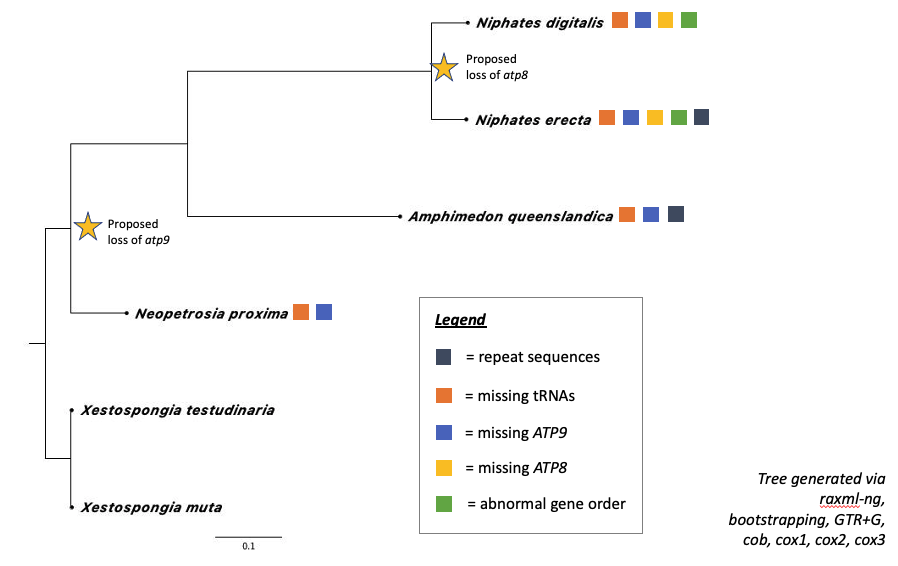
\includegraphics[width=1.0\textwidth]{Figures/figure 7.png}
    \caption{Phylogenetic tree of Clade B generated with raxml-ng, GTR+G, and using \emph{cob, cox1, cox2, and cox3}.}
\end{figure}
\end{document}